\documentclass[12pt]{article}
\usepackage{graphicx}
\usepackage[explicit]{titlesec}	
\usepackage{blindtext}
\usepackage{amsthm}
\usepackage{amssymb}
\usepackage{mathtools}
\usepackage{anyfontsize}
\usepackage{xstring}
\usepackage{xargs}
\usepackage{makeidx}
\usepackage{cancel}
\usepackage{fancyhdr}
\usepackage{chngcntr}
\usepackage{caption}
\usepackage{subcaption}
\usepackage{float}
\usepackage{pgf,tikz,pgfplots}
\usepackage{latexsym}
\usepackage{verbatim}
\usepackage{enumitem,amsmath,array}
\usepackage{tkz-graph}
\usepackage{bookmark}
\usepackage{csquotes}
\usetikzlibrary{positioning,chains,fit,shapes,calc,decorations.markings,decorations.pathreplacing,arrows.meta}
\usepackage[a4paper,left=2cm,right=2cm,top=3cm,bottom=2.4cm]{geometry}
\usepackage{listings}
%\usepackage{clrscode3e}
\usepackage{hyperref}
\hypersetup{
	colorlinks=true,
	linkcolor=blue,
	filecolor=magenta,      
	urlcolor=cyan,
}

\usepackage[]{xepersian}
\usepackage{bidicontour}
\usepackage{bidi}
\bidicontourlength{1pt}

\settextfont[BoldFont=HM XNiloofarBd.ttf, ItalicFont=HM XNiloofarIt.ttf, BoldItalicFont=HM XNiloofarBdIt.ttf]{HM XNiloofar.ttf}
\setdigitfont[BoldFont=HM XNiloofarBd.ttf, ItalicFont=HM XNiloofarIt.ttf, BoldItalicFont=HM XNiloofarBdIt.ttf]{HM XNiloofar.ttf}

\ExplSyntaxOn
\cs_new_eq:NN \calc \fp_eval:n
\ExplSyntaxOff

\setlength{\parindent}{1.5em}
\setlength{\parskip}{0.9em}
\renewcommand{\baselinestretch}{1.4}

\def\chapterfont{25}

\newcounter{mytheorem}
\newcounter{mysection}
\counterwithin{figure}{section}

\fancypagestyle{mypagestyle}{%
	\fancyfoot{}
	\fancyhf{}
	\fancyhead[R]{}
	\fancyhead[L]{}
	\fancyfoot[C]{\thepage}
	\renewcommand{\headrulewidth}{0pt}
}
\pagestyle{mypagestyle}

\makeatletter
\renewcommand\section{\@startsection {section}{1}{0pt}%
	{3.5ex plus 1ex minus .2ex}%
	{2.3ex plus .2ex}%
	{\setcounter{equation}{0}\setcounter{mytheorem}{0}\normalfont\Large\bfseries}}
\makeatother

\renewcommand\theequation{\thesection.\arabic{equation}}
\renewcommand\themytheorem{\thesection.\arabic{mytheorem}}


\newenvironment{mytheorem}[1]{\refstepcounter{mytheorem} \vspace*{.2cm}\noindent
	\textbf{قضیه‌ی \themytheorem \ #1}\itshape
}{}

\newenvironment{mylemma}[1]{\refstepcounter{mytheorem} \vspace*{.2cm}\noindent
	\textbf{لم \themytheorem \ #1}\itshape
}{}

\newenvironment{mydef}[1]{\refstepcounter{mytheorem} \vspace*{.2cm}\noindent
	\textbf{تعریف \themytheorem \ #1}\ \itshape
}{}

\newenvironment{myprop}[1]{\refstepcounter{mytheorem} \vspace*{.2cm}\noindent
	\textbf{گزاره‌ی \themytheorem \ #1}\itshape
}{}

\newenvironment{mymol}[1]{\refstepcounter{mytheorem} \vspace*{.2cm}\noindent
	\textbf{ملاحظه‌ی \themytheorem \ #1}\itshape
}{}

\newenvironment{mynat}[1]{\refstepcounter{mytheorem} \vspace*{.2cm}\noindent
	\textbf{نتیجه‌ی \themytheorem \ #1}\itshape
}{}

\newenvironment{myprob}[1]{\refstepcounter{mytheorem} \vspace*{.2cm}\noindent
	\textbf{مسئله‌ی \themytheorem \ #1}\itshape
}{}

\newenvironment{myguess}[1]{\refstepcounter{mytheorem} \vspace*{.2cm}\noindent
	\textbf{حدس \themytheorem \ #1}\itshape
}{}

\newenvironment{example}
{\smallskip \noindent \emph{مثال:}}
{\hfill $\boxtimes$ \smallskip}

\newenvironment{myproof}{\noindent\textit{برهان.}}{\hfill $\square$}

\newcommand{\set}[2]{\left\{#1 \ \middle|\ #2\right\}}
\newcommand{\seq}[4]{%
	\IfEqCase{#4}{%
		{var}{\left\{#1_{#2},#1_{#2+1},\dots,#1_{#3}\right\}}
		{num}{\left\{#1_{#2},#1_{\calc{#2+1}},\dots,#1_{#3}\right\}}
	}
}
\newcommand{\te}[1]{\text{\lr{#1}}}
\newcommand{\trans}[2]{#1\LTRfootnote{#2}}

\title{گزارش فاز اول پروژه یادگیری ماشین در فیزیک}
\author{روژین محمدی کیان، علی ابوالحسن‌زاده ماهانی، فاطمه سلیمانی مقدم، علی قبله}

\begin{document}
\maketitle
\section{گزارش اولیه:}
بهمن نورونی، پدیده‌ای است که رفتار جمعی نورون‌ها را توصیف می‌کند. رفتار هر نورون منفرد روی نورون‌های اطرافش تاثیر می‌گذارد. در حالت کلی، 3 رویداد را می‌توان برای نورون‌ها متصور شد، حالت پیش‌بحرانی که هر نورون به طور میانگین کمتر از یک نورون دیگر را روشن می‌کند، حالت بحرانی که میانگین نورون‌های روشن شده یک است و حالت پسابحرانی هم هر نورون به طور میانگین بیش از یک نورون دیگر را روشن می‌کند.
شکل نمودار (log-log) در حالت بحرانی به صورت خطی است اما در حالت کلی به دلیل برخی محدودیت‌ها این نمودار افت ناگهانی پیدا می‌‌کند که تشخیص بحرانی بودن یا نبودن نمودار را دشوار می‌کند.
\\
داده‌های اولیه‌ی پروژه، که قرار است برای تشخیص بحرانی بودن یا نبودن نمودار استفاده شود، قبلتر توسط آقای نقی‌لو شبیه‌سازی شده‌بودند. داده‌های خام به صورت مجموعه‌ای از آرایه‌ها بودند که احتمال وقوع بهمن را بر حسب اندازه آن بیان می‌کردند. مشکل ابتدایی داده‌ها این بود که سبدبندی نشده‌بودند که کد سبدبندی آن‌ها نیز ضمیمه شده‌است.
\\
یک نمونه نمودار برای داده‌های سبدبندی نشده(راست) و سبدبندی شده(چپ) به شکل زیر است:
\\
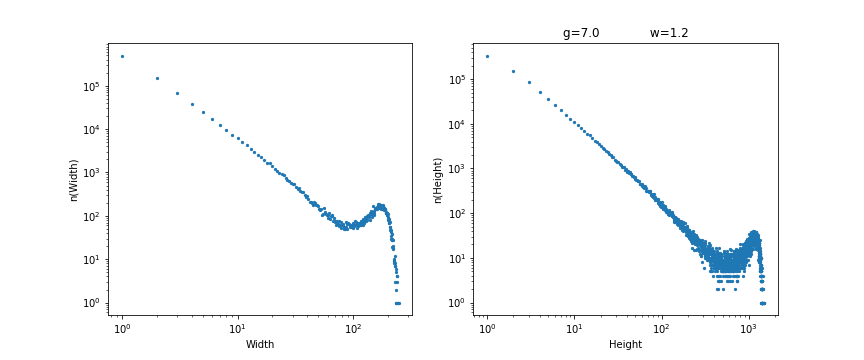
\includegraphics[scale=0.5]{g7.0 w1.2 base1 P}
\\
بعد داده‌ها بعد از سبدبندی حدود 90 در 9000 بود.
\\
\\
از آن‌جایی که داده‌های اولیه برچسب‌گذاری نشده‌بودند، مرحله بعدی کار برچسب‌گذاری داده‌ها با توجه به ویژگی‌های سیستم بود. درشکل بالا توزیع هر کدام از نمودارها بر حسب پارامترهای $w$ و $base$ رسم شده‌است. ناحیه زرد بیانگر نمودارهای فرابحرانی، ناحیه سبز بحرانی و ناحیه آبی فروبحرانی است.
\\

\begin{figure}[t]
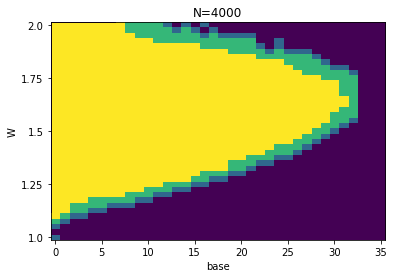
\includegraphics[width=8cm]{n4000}
\centering
\end{figure}
\\
به دلیل اینکه پس از سبدبندی هم بعد ماتریس داده‌ها بسیار زیاد بود، باید تعدادی خصیصه از بین داده‌ها پیدا می‌کردیم، با توجه به فرم کلی نمودارها در هر حالت بحرانی، فرابحرانی و فروبحرانی، ویژگی‌های مدنظر شامل تقعر نمودار، تعداد نقاط عطف، تعداد نقاط اکسترمم، اختلاف ارتفاع کمینه و بیشینه موضعی و تابعی برحسب مقدار متوسط توان‌های مختلف بزرگی بهمن بودند.
\\
بعد داده‌های نهایی پس از استخراج ویژگی‌ها 12 در 8798 است.

\section{منابع:}

\begin{flushleft}
$1-John M. Beggs (2007). Neuronal avalanche. Scholarpedia. 2(1):1344. doi:10.4249/scholarpedia.1344:$
\end{flushleft}
\\
در این مقاله، توضیحات اولیه درباره بهمن‌های نورونی، نحوه رخدادن بهمن‌ها و حالت فرابحرانی، فروبحرانی و بحرانی داده‌شده‌است.
\\
\begin{flushleft}
$2-Amin Safaeesirat, Saman Moghimi-Araghi. Critical behaviour at the onset of synchronization in a neuronal model. arXiv:2010.01493v2:$
\end{flushleft}
\\
این مقاله ابتدا با مطالعه‌ی رفتار یک تک نورون، سپس مجموعه‌ای از نورون‌ها، یک نمونه رفتار بحرانی را برای شبکه عصبی بررسی کرده‌است.
\\
به نوعی دو مقاله بالا، درباره‌ی رفتار بحرانی شبکه‌های عصبی بودند، همچنین در روند انجام پروژه از کارهای آقای نقی‌لو هم استفاده شد که هنوز مقاله نشده‌اند.
\\
\begin{flushleft}
$G. Pruessner.(2012).$
\\
$Self-Organised Criticality theory, Models and Characterisation.Cambridge:$
\end{flushleft}
\\
این کتاب، به خصوص دو فصل ابتدایی آن برای شناخت بیشتر پدیده‌های بحرانی، و بهمن‌ها مفید بود.
\\
\end{document}